% Shared preamble for the multilayer-perceptron exercises.
% Each exercise is a standalone document: compile it from this directory.
\documentclass[11pt,a4paper]{article}

\usepackage[margin=2.35cm,top=1.85cm,bottom=2.15cm,headheight=22pt,headsep=9pt]{geometry}
\usepackage[T1]{fontenc}
\usepackage[utf8]{inputenc}
\usepackage[english]{babel}
\usepackage{lmodern}
\usepackage{textcomp}
\usepackage{microtype}
\usepackage{amsmath,amssymb,amsthm,mathtools}
\usepackage{booktabs}
\usepackage{array}
\usepackage{enumitem}
\usepackage{xcolor}
\usepackage{tikz}
\usetikzlibrary{arrows.meta,positioning,calc}
\usepackage{pgfplots}
\pgfplotsset{compat=1.17}
\usepackage[hypcap=false]{caption}
\usepackage{needspace}
\usepackage{titlesec}
\usepackage{fancyhdr}
\usepackage[hidelinks,unicode]{hyperref}

\setlength{\parindent}{1.15em}
\setlength{\parskip}{0pt}
\setlength{\abovedisplayskip}{7pt plus 2pt minus 2pt}
\setlength{\belowdisplayskip}{7pt plus 2pt minus 2pt}
\setlength{\abovedisplayshortskip}{4pt plus 2pt}
\setlength{\belowdisplayshortskip}{5pt plus 2pt}
\setlength{\emergencystretch}{2em}
\allowdisplaybreaks[1]

\definecolor{navy}{HTML}{1B365D}
\definecolor{ink}{HTML}{1C1917}
\definecolor{rulegold}{HTML}{8C6A32}
\definecolor{wash}{HTML}{F6F3EC}
\definecolor{accent}{HTML}{7A2E2E}

\pagestyle{fancy}
\fancyhf{}
\fancyhead[L]{\small\sffamily\color{navy}Universidad Pontificia Comillas}
\fancyhead[R]{\small\sffamily\color{navy}\exerciseshort}
\fancyfoot[C]{\small\color{ink!70}\thepage}
\renewcommand{\headrulewidth}{0.4pt}
\renewcommand{\headrule}{%
  \hbox to\headwidth{\color{rulegold}\leaders\hrule height \headrulewidth\hfill}%
}
\fancypagestyle{plain}{%
  \fancyhf{}%
  \fancyfoot[C]{\small\color{ink!70}\thepage}%
  \renewcommand{\headrulewidth}{0pt}%
}

\captionsetup{
  font={small},
  labelfont={sf,bf,color=navy},
  labelsep=period,
  skip=7pt
}

\titleformat{\section}
  {\Large\bfseries\sffamily\color{navy}}
  {\thesection}{0.55em}{}
  [\vspace{0.2em}{\color{navy}\titlerule[0.55pt]}]
\titleformat{\subsection}
  {\normalsize\bfseries\sffamily\color{navy}}
  {}{0pt}{}
  [\vspace{-0.15em}{\color{rulegold}\titlerule[0.4pt]}]
\titlespacing*{\section}{0pt}{1.15em}{0.55em}
\titlespacing*{\subsection}{0pt}{1.05em}{0.4em}

\theoremstyle{plain}
\newtheorem{lemma}{Lemma}
\newtheorem{proposition}{Proposition}
\theoremstyle{definition}
\newtheorem*{remark}{Remark}

\setlist[enumerate]{leftmargin=1.7em,itemsep=0.5em,topsep=0.35em,labelsep=0.5em}
\setlist[itemize]{leftmargin=1.35em,itemsep=0.25em,topsep=0.3em}

\newcommand{\exerciseshort}{Multilayer perceptrons}
\newcommand{\R}{\mathbb{R}}
\newcommand{\E}{\mathbb{E}}
\DeclareMathOperator{\Var}{Var}
\DeclareMathOperator{\relu}{ReLU}
\DeclarePairedDelimiter{\abs}{\lvert}{\rvert}
\DeclarePairedDelimiter{\norm}{\lVert}{\rVert}
\newcommand{\dd}{\mathrm{d}}
\newcommand{\T}{\mathsf{T}}

\tikzset{
  neuron/.style={
    circle, draw=navy, line width=0.65pt, minimum size=8.2mm,
    inner sep=0pt, font=\small, fill=white
  },
  ninput/.style={neuron, fill=navy!6},
  nhidden/.style={neuron, fill=navy!11},
  noutput/.style={neuron, fill=rulegold!18},
  ndead/.style={neuron, fill=ink!8, draw=ink!45, text=ink!55},
  nedge/.style={
    -{Stealth[length=1.65mm,width=1.35mm]},
    draw=ink!72, line width=0.45pt
  },
  ntag/.style={font=\scriptsize\sffamily, text=navy}
}

% #1 number, #2 running head, #3 display title, #4 introductory paragraph
\newcommand{\exercisefront}[4]{%
  \thispagestyle{plain}%
  \gdef\exerciseshort{Exercise #1\enspace\textperiodcentered\enspace #2}%
  \noindent{\sffamily\footnotesize\color{navy}%
    \MakeUppercase{Universidad Pontificia Comillas}}\par
  \vspace{0.15em}
  \noindent{\sffamily\footnotesize\color{ink!80}%
    Teaching collection of Eduardo C\'esar Garrido Merch\'an}\par
  \vspace{0.55em}
  \noindent{\sffamily\small\color{ink!75}%
    Multilayer perceptrons%
    \enspace\textcolor{rulegold}{\textperiodcentered}\enspace
    Exercise #1 of 3}\par
  \vspace{0.7em}
  \noindent{\sffamily\LARGE\bfseries\color{navy}#3\par}
  \vspace{0.35em}
  \noindent{\color{rulegold}\rule{\textwidth}{0.7pt}}\par
  \vspace{0.75em}
  \noindent #4\par
  \vspace{0.15em}
}

\newcommand{\solutionpart}[1]{%
  \Needspace{8\baselineskip}%
  \subsection*{Solution to (#1)}%
}

\hypersetup{
  pdfauthor={Eduardo C\'esar Garrido Merch\'an},
  pdfsubject={Graduate exercises on multilayer perceptrons}
}

\hypersetup{pdftitle={Exercise 1. Forward propagation and backpropagation}}

\begin{document}

\exercisefront{1}{Backpropagation}
  {Forward propagation and backpropagation}
  {This exercise asks for the forward and backward pass of a small multilayer perceptron, first for one training pair and then in matrix form for a minibatch. The calculus is the chain rule; the linear algebra is there to keep the shapes honest. A calculator is appropriate for the logistic function. Every derivative should be derived, not quoted from a library.}

\section{Setup}

Consider a network with input dimension \(2\), one hidden layer of width \(2\), and a scalar output. Both layers use the logistic sigmoid
\[
  \sigma(t) = \frac{1}{1+e^{-t}},
  \qquad
  \sigma'(t) = \sigma(t)\bigl(1-\sigma(t)\bigr),
\]
applied elementwise to vectors. For an input \(x\in\R^2\) and a target \(y\in\R\),
\begin{align}
  z^{(1)} &= W^{(1)} x + b^{(1)}, &
  a^{(1)} &= \sigma\bigl(z^{(1)}\bigr), \label{eq:forward-hidden}\\
  z^{(2)} &= W^{(2)} a^{(1)} + b^{(2)}, &
  \hat y &= \sigma\bigl(z^{(2)}\bigr), \label{eq:forward-out}\\
  L &= \tfrac12\bigl(\hat y - y\bigr)^2. \label{eq:mse}
\end{align}
The parameters of the worked example are
\begin{align*}
  W^{(1)} &= \begin{pmatrix} 0.5 & -0.2 \\ 0.1 & 0.3 \end{pmatrix},
  &
  b^{(1)} &= \begin{pmatrix} 0.1 \\ -0.1 \end{pmatrix},
  \\[0.4em]
  W^{(2)} &= \begin{pmatrix} 0.4 & -0.5 \end{pmatrix},
  &
  b^{(2)} &= 0.2,
\end{align*}
and the training pair is \(x = (1,\, 0)^\T\), \(y = 1\). Hidden units are written \(h_1,h_2\) in the diagram; their values are the coordinates of \(a^{(1)}\).

\begin{center}
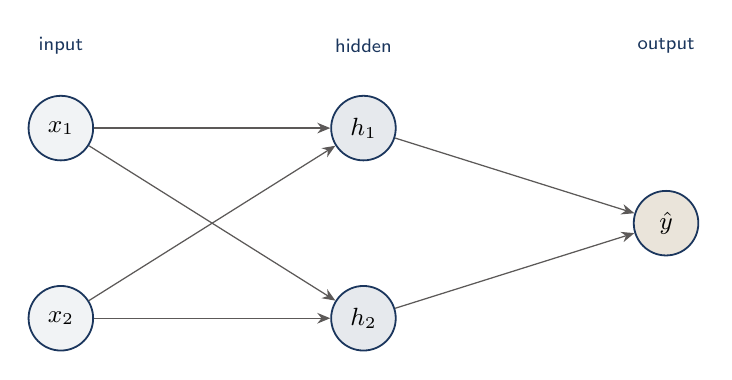
\begin{tikzpicture}[x=1.22cm,y=1.05cm]
  \node[ninput] (x1) at (0, 1.15) {$x_1$};
  \node[ninput] (x2) at (0,-1.15) {$x_2$};
  \node[nhidden] (h1) at (3.15, 1.15) {$h_1$};
  \node[nhidden] (h2) at (3.15,-1.15) {$h_2$};
  \node[noutput] (yhat) at (6.3,0) {$\hat y$};
  \draw[nedge] (x1) -- (h1);
  \draw[nedge] (x1) -- (h2);
  \draw[nedge] (x2) -- (h1);
  \draw[nedge] (x2) -- (h2);
  \draw[nedge] (h1) -- (yhat);
  \draw[nedge] (h2) -- (yhat);
  \node[ntag] at (0,2.15) {input};
  \node[ntag] at (3.15,2.15) {hidden};
  \node[ntag] at (6.3,2.15) {output};
\end{tikzpicture}
\captionof{figure}{The \(2\)--\(2\)--\(1\) network. Biases are omitted from the drawing and appear in \eqref{eq:forward-hidden}--\eqref{eq:forward-out}.}
\label{fig:net}
\end{center}

Throughout, vectors are columns. The gradient of a scalar with respect to a matrix \(W\) is the matrix of partial derivatives, of the same shape as \(W\). The symbol \(\odot\) denotes the elementwise (Hadamard) product.

\section{Questions}

\begin{enumerate}[label=\textbf{(\alph*)}]
  \item Write the forward computation in the shapes of \eqref{eq:forward-hidden}--\eqref{eq:mse} and evaluate \(z^{(1)}\), \(a^{(1)}\), \(z^{(2)}\), \(\hat y\), and \(L\) to six decimal places.

  \item Let \(\delta^{(2)} = \partial L/\partial z^{(2)}\), a scalar. Derive
  \[
    \frac{\partial L}{\partial W^{(2)}} = \delta^{(2)}\bigl(a^{(1)}\bigr)^\T,
    \qquad
    \frac{\partial L}{\partial b^{(2)}} = \delta^{(2)}
  \]
  from the chain rule, and evaluate both quantities.

  \item Show that the Jacobian of \(u\mapsto \sigma(u)\) at \(z^{(1)}\) is diagonal. Deduce
  \[
    \delta^{(1)}
    =
    \bigl(W^{(2)}\bigr)^\T \delta^{(2)} \odot \sigma'\bigl(z^{(1)}\bigr)
    \in \R^2
  \]
  and the hidden-layer gradients
  \[
    \frac{\partial L}{\partial W^{(1)}} = \delta^{(1)} x^\T,
    \qquad
    \frac{\partial L}{\partial b^{(1)}} = \delta^{(1)}.
  \]
  Evaluate them, and explain the zero pattern in \(\partial L/\partial W^{(1)}\) without referring to the numerical values of the sigmoids.

  \item Now let a minibatch consist of \(N\) examples stored as columns of \(X\in\R^{d_0\times N}\), and let the training objective be the average of the per-example losses. For each layer \(\ell\), with preactivations \(Z^{(\ell)}\) and activations \(A^{(\ell)}\) likewise stored by columns, prove
  \begin{equation}
    \frac{\partial L}{\partial W^{(\ell)}}
    =
    \frac1N \Delta^{(\ell)}\bigl(A^{(\ell-1)}\bigr)^\T,
    \qquad
    \frac{\partial L}{\partial b^{(\ell)}}
    =
    \frac1N \Delta^{(\ell)}\mathbf{1},
    \label{eq:batch}
  \end{equation}
  where column \(n\) of \(\Delta^{(\ell)}\) is the gradient of the \emph{per-example} loss with respect to \(z^{(\ell)}_n\), and \(\mathbf{1}\in\R^N\) is the all-ones vector. Then specialise the output factor: for the squared loss \eqref{eq:mse} it retains a factor \(\sigma'(z)\), whereas for the binary cross-entropy
  \[
    \ell(\hat y, y)
    =
    -\, y\log\hat y - (1-y)\log(1-\hat y)
  \]
  with \(\hat y = \sigma(z)\) and \(y\in\{0,1\}\), the output delta collapses to \(\hat y - y\).

  \item Let \(\theta\) collect every parameter and let \(g = \nabla_\theta L(\theta)\). Define \(\varphi(\eta) = L(\theta - \eta g)\). Show that \(\varphi'(0) = -\norm{g}_2^2\), and conclude that if \(g\neq 0\) then every sufficiently small positive step strictly decreases \(L\). For the numerical network, take \(\eta = 1/2\), report the updated parameters to six decimal places, recompute the loss, and check the decrease against the first-order prediction \(\eta\norm{g}_2^2\).
\end{enumerate}

The worked solution begins on the next page.

\clearpage
\section{Solutions}

Numerical entries below are correctly rounded to six decimal places from double-precision evaluation. Every nonzero partial derivative agrees with a central difference of step \(10^{-6}\) to a relative error below \(10^{-9}\). The structural zeros are exact.

\solutionpart{a}

The shapes are those in \eqref{eq:forward-hidden}--\eqref{eq:mse}: \(W^{(1)}\in\R^{2\times 2}\), \(b^{(1)}\in\R^2\), \(W^{(2)}\in\R^{1\times 2}\), and \(b^{(2)}\in\R\). Substituting the given sample,
\[
  z^{(1)}
  =
  \begin{pmatrix} 0.5 & -0.2 \\ 0.1 & 0.3 \end{pmatrix}
  \begin{pmatrix} 1 \\ 0 \end{pmatrix}
  +
  \begin{pmatrix} 0.1 \\ -0.1 \end{pmatrix}
  =
  \begin{pmatrix} 0.6 \\ 0 \end{pmatrix}.
\]
The second coordinate vanishes because it is the second standard basis direction: only the first column of \(W^{(1)}\) meets a nonzero input. Then
\[
  a^{(1)}
  =
  \begin{pmatrix} \sigma(0.6) \\ \sigma(0) \end{pmatrix}
  =
  \begin{pmatrix} 0.645656 \\ 0.500000 \end{pmatrix},
\]
since \(\sigma(0) = 1/2\) exactly and \(\sigma(0.6) = 0.645656306\ldots\). The output preactivation is
\begin{align*}
  z^{(2)}
  &= 0.4\cdot 0.645656306 - 0.5\cdot 0.5 + 0.2 \\
  &= 0.208262522,
\end{align*}
so \(z^{(2)} = 0.208263\) to six decimals, and
\[
  \hat y = \sigma\bigl(z^{(2)}\bigr) = 0.551878,
  \qquad
  L = \tfrac12\bigl(0.551878255 - 1\bigr)^2 = 0.100407.
\]
The prediction sits well below the target, which will determine the sign of every output-layer derivative.

\solutionpart{b}

Differentiate the scalar map \(z^{(2)} = W^{(2)} a^{(1)} + b^{(2)}\) with \(a^{(1)}\) held fixed. If \(W^{(2)} = (w_1,\, w_2)\) and \(a^{(1)} = (a_1,\, a_2)^\T\), then \(z^{(2)} = w_1 a_1 + w_2 a_2 + b^{(2)}\), so
\[
  \frac{\partial z^{(2)}}{\partial w_j} = a_j,
  \qquad
  \frac{\partial z^{(2)}}{\partial b^{(2)}} = 1.
\]
The chain rule through \(L\) contributes the same upstream factor \(\delta^{(2)} = \partial L/\partial z^{(2)}\) to each parameter, and the two partials in \(w\) assemble into the outer product \(\delta^{(2)}(a^{(1)})^\T\). In differential notation, \(\dd z^{(2)} = \dd W^{(2)}\, a^{(1)} + \dd b^{(2)}\) and
\[
  \dd L = \delta^{(2)}\,\dd z^{(2)}
  = \bigl\langle \delta^{(2)}(a^{(1)})^\T,\, \dd W^{(2)}\bigr\rangle_F
  + \delta^{(2)}\,\dd b^{(2)},
\]
which is the same identity. For the squared loss,
\[
  \frac{\partial L}{\partial \hat y} = \hat y - y,
  \qquad
  \delta^{(2)} = (\hat y - y)\,\sigma'\bigl(z^{(2)}\bigr).
\]
Numerically \(\hat y - y = -0.448122\) and
\[
  \sigma'\bigl(z^{(2)}\bigr) = \hat y(1-\hat y) = 0.247309,
\]
hence \(\delta^{(2)} = -0.110824\). The minus sign says that increasing \(z^{(2)}\) decreases \(L\), as it must while \(\hat y < y\). Therefore
\begin{align*}
  \frac{\partial L}{\partial W^{(2)}}
  &=
  -0.110824\cdot\begin{pmatrix} 0.645656 & 0.500000 \end{pmatrix}
  =
  \begin{pmatrix} -0.071554 & -0.055412 \end{pmatrix},
  \\[0.3em]
  \frac{\partial L}{\partial b^{(2)}}
  &= -0.110824.
\end{align*}

\solutionpart{c}

Write \(\sigma(u)_i = \sigma(u_i)\). Then
\[
  \frac{\partial \sigma(u)_i}{\partial u_j}
  =
  \sigma'(u_i)\,\mathbf{1}_{\{i=j\}},
\]
so the Jacobian \(D\sigma(z^{(1)})\) is the diagonal matrix \(\operatorname{diag}\bigl(\sigma'(z^{(1)})\bigr)\). No hidden unit's output depends on another unit's preactivation.

The output preactivation depends on the hidden activation through \(z^{(2)} = W^{(2)} a^{(1)} + b^{(2)}\). With \(W^{(2)}\) a row, the gradient of \(z^{(2)}\) with respect to the column \(a^{(1)}\) is \((W^{(2)})^\T\). The chain rule from \(z^{(2)}\) down to \(z^{(1)}\) is therefore
\begin{equation}
  \delta^{(1)}
  =
  \frac{\partial L}{\partial z^{(1)}}
  =
  D\sigma\bigl(z^{(1)}\bigr)^\T
  \bigl(W^{(2)}\bigr)^\T
  \delta^{(2)}.
  \label{eq:delta1}
\end{equation}
The Jacobian is symmetric, and multiplication by a diagonal matrix is the Hadamard product with its diagonal, which is \eqref{eq:delta1} in the form requested. Explicitly,
\[
  \bigl(W^{(2)}\bigr)^\T\delta^{(2)}
  =
  \begin{pmatrix} 0.4 \\ -0.5 \end{pmatrix}(-0.110824)
  =
  \begin{pmatrix} -0.044330 \\ 0.055412 \end{pmatrix}.
\]
The hidden derivatives are \(\sigma'(0.6) = 0.228784\) and \(\sigma'(0) = 1/4\), so
\[
  \delta^{(1)}
  =
  \begin{pmatrix} -0.044330\cdot 0.228784 \\ 0.055412\cdot 0.25 \end{pmatrix}
  =
  \begin{pmatrix} -0.010142 \\ 0.013853 \end{pmatrix}.
\]
The same outer-product argument as in (b), now with incoming activation \(x\), gives
\[
  \frac{\partial L}{\partial W^{(1)}}
  =
  \delta^{(1)} x^\T
  =
  \begin{pmatrix} -0.010142 \\ 0.013853 \end{pmatrix}
  \begin{pmatrix} 1 & 0 \end{pmatrix}
  =
  \begin{pmatrix}
    -0.010142 & 0 \\
    0.013853 & 0
  \end{pmatrix},
\]
and \(\partial L/\partial b^{(1)} = \delta^{(1)}\).

The second column is zero for a structural reason. The forward map uses \(W^{(1)}\) only through the product \(W^{(1)}x\). Differentiating in an entry \(W^{(1)}_{ij}\) produces a multiple of the coordinate \(x_j\). Here \(x_2 = 0\), so every weight that multiplies \(x_2\) can be changed without changing \(z^{(1)}\), \(a^{(1)}\), \(\hat y\), or \(L\). Those partial derivatives vanish before any activation is evaluated. A nonzero input coordinate would not have produced this column of zeros; saturation of \(\sigma\) is a different phenomenon, visible here only in the magnitudes of \(\sigma'\).

\solutionpart{d}

\paragraph{Minibatch outer products.}
Let \(\ell_n\) be the loss of example \(n\), and let \(L = N^{-1}\sum_{n=1}^N \ell_n\). Write \(A^{(0)} = X\) and
\[
  Z^{(\ell)} = W^{(\ell)} A^{(\ell-1)} + b^{(\ell)}\mathbf{1}^\T,
  \qquad
  A^{(\ell)} = \sigma\bigl(Z^{(\ell)}\bigr),
\]
with \(\sigma\) applied elementwise. Let \(S = \sum_n \ell_n\), and let column \(n\) of \(\Delta^{(\ell)}\) be \(\partial \ell_n/\partial z^{(\ell)}_n\). The scalar \(S\) depends on the preactivation matrix through
\[
  \dd S = \bigl\langle \Delta^{(\ell)},\, \dd Z^{(\ell)}\bigr\rangle_F
\]
when the differential is taken at layer \(\ell\), because each column contributes its own inner product and distinct examples do not share preactivations. Holding the incoming activation fixed,
\[
  \dd Z^{(\ell)} = \dd W^{(\ell)}\, A^{(\ell-1)} + \dd b^{(\ell)}\,\mathbf{1}^\T.
\]
The Frobenius identity \(\langle \Delta,\, \dd W\, A\rangle_F = \langle \Delta A^\T,\, \dd W\rangle_F\) then yields
\[
  \frac{\partial S}{\partial W^{(\ell)}} = \Delta^{(\ell)}\bigl(A^{(\ell-1)}\bigr)^\T,
  \qquad
  \frac{\partial S}{\partial b^{(\ell)}} = \Delta^{(\ell)}\mathbf{1}.
\]
Dividing by \(N\) is \eqref{eq:batch}. The recurrence that builds \(\Delta^{(\ell)}\) from \(\Delta^{(\ell+1)}\) is the columnwise form of \eqref{eq:delta1},
\[
  \Delta^{(\ell)}
  =
  \Bigl(\bigl(W^{(\ell+1)}\bigr)^\T \Delta^{(\ell+1)}\Bigr)
  \odot \sigma'\bigl(Z^{(\ell)}\bigr),
\]
with the output case supplied by the choice of \(\ell_n\). The factor \(1/N\) is not part of this recurrence: it appears once, when the averaged objective differentiates with respect to a parameter.

One orientation warning is worth recording. The convention here stores one example per column, so the activation matrix is features-by-batch. Implementations that store one example per row use the transposed product, with the factor \(1/N\) unchanged.

\paragraph{Squared loss and cross-entropy.}
For \(\ell = \tfrac12(\hat y - y)^2\) and \(\hat y = \sigma(z)\),
\[
  \frac{\partial \ell}{\partial z} = (\hat y - y)\,\sigma'(z),
\]
which is the output column of \(\Delta^{(L)}\). For binary cross-entropy, differentiate in \(\hat y\) first:
\[
  \frac{\partial \ell}{\partial \hat y}
  =
  -\frac{y}{\hat y} + \frac{1-y}{1-\hat y}
  =
  \frac{\hat y - y}{\hat y\,(1-\hat y)},
\]
provided \(\hat y\in(0,1)\). Multiply by \(\sigma'(z) = \hat y(1-\hat y)\):
\begin{equation}
  \frac{\partial \ell}{\partial z}
  =
  \frac{\hat y - y}{\hat y\,(1-\hat y)}\cdot \hat y\,(1-\hat y)
  =
  \hat y - y.
  \label{eq:bce-delta}
\end{equation}
The sigmoid derivative cancels, including at the saturated tails where \(\sigma'(z)\) itself underflows. The same algebra holds for a soft target \(y\in(0,1)\); the hypothesis \(y\in\{0,1\}\) is only the classification interpretation. Combining \eqref{eq:bce-delta} with \eqref{eq:batch}, a sigmoid output trained by mean binary cross-entropy has
\[
  \frac{\partial L}{\partial W^{(L)}}
  =
  \frac1N (\hat y - y)\,\bigl(A^{(L-1)}\bigr)^\T
\]
in the scalar-output case, with \(\hat y - y\) the row of residuals. The squared loss keeps an extra diagonal factor \(\sigma'(z^{(L)})\) and is therefore more prone to stalling once the output saturates. That comparison is continued, for deep sigmoid stacks, in Exercise~3.

\solutionpart{e}

The map \(\varphi\) is the composition of \(L\) with the affine path \(\eta\mapsto \theta - \eta g\). The chain rule in several variables gives
\[
  \varphi'(0)
  =
  \bigl\langle \nabla L(\theta),\, -g\bigr\rangle
  =
  -\langle g, g\rangle
  =
  -\norm{g}_2^2.
\]
If \(g\neq 0\), then \(\varphi'(0) < 0\). By the definition of the derivative there exists \(\eta_0>0\) such that
\[
  \frac{\varphi(\eta)-\varphi(0)}{\eta} < 0
  \qquad\text{for all }\eta\in(0,\eta_0),
\]
hence \(\varphi(\eta) < \varphi(0)\). Differentiability of \(L\), which holds here because \(\sigma\) is \(C^\infty\), is the only regularity used. No global smoothness constant is required for a sufficiently small step.

On the numerical example the parameter gradient is not zero: already \(\partial L/\partial b^{(2)} = -0.110824\). Its squared Euclidean norm, summing the squares of all nine scalar partials computed in (b) and (c), is
\[
  \norm{g}_2^2 = 0.021062.
\]
The step \(\eta = 1/2\) therefore has first-order predicted decrease \(\eta\norm{g}_2^2 = 0.010531\). The updated parameters are
\begin{align*}
  W^{(1)} &\leftarrow
  \begin{pmatrix}
    0.505071 & -0.200000 \\
    0.093073 & 0.300000
  \end{pmatrix},
  &
  b^{(1)} &\leftarrow
  \begin{pmatrix} 0.105071 \\ -0.106927 \end{pmatrix},
  \\[0.35em]
  W^{(2)} &\leftarrow
  \begin{pmatrix} 0.435777 & -0.472294 \end{pmatrix},
  &
  b^{(2)} &\leftarrow 0.255412.
\end{align*}
The second column of \(W^{(1)}\) is unchanged, as its gradient vanished. The new forward pass on the same pair is
\begin{align*}
  z^{(1)} &= \begin{pmatrix} 0.610142 \\ -0.013853 \end{pmatrix},
  &
  a^{(1)} &= \begin{pmatrix} 0.647973 \\ 0.496537 \end{pmatrix},
  \\
  z^{(2)} &= 0.303273,
  &
  \hat y &= 0.575242,
  &
  L &= 0.090210.
\end{align*}
The loss falls from \(0.100407\) to \(0.090210\), a decrease of \(0.010197\). The gap between this value and the predicted \(0.010531\) is the usual second-order remainder: the first-order calculation uses the gradient at the old point, and \(L\) is not linear. The sign agrees, and \(\eta = 1/2\) is inside the descent range for this particular loss.

\begin{thebibliography}{9}
\bibitem{rumelhart1986}
D.~E. Rumelhart, G.~E. Hinton, and R.~J. Williams.
\newblock Learning representations by back-propagating errors.
\newblock \emph{Nature}, 323:533--536, 1986.

\bibitem{goodfellow2016}
I.~Goodfellow, Y.~Bengio, and A.~Courville.
\newblock \emph{Deep Learning}. MIT Press, 2016.
\newblock Chapter~6 treats the same back-propagation identities in the column-vector convention used here.
\end{thebibliography}

\end{document}
